
\chapter{显著性区域检测基础}
在本章中,将分类介绍国际上主流的几类显著区域检测方法:基于局部对比度(MZ\cite{ma2003contrast}),基于全局对比度(HC,RC\cite{cheng2011global}),基于频域分析(SR\cite{hou2007saliency}),基于学习(CRF\cite{maisaliency})。随后,还介绍了近年来的一些最新工作和研究趋势,并以此为基础,确定了本文的研究思路和框架。

\section{基于局部对比度的方法}
\begin{figure}[h]
\centering
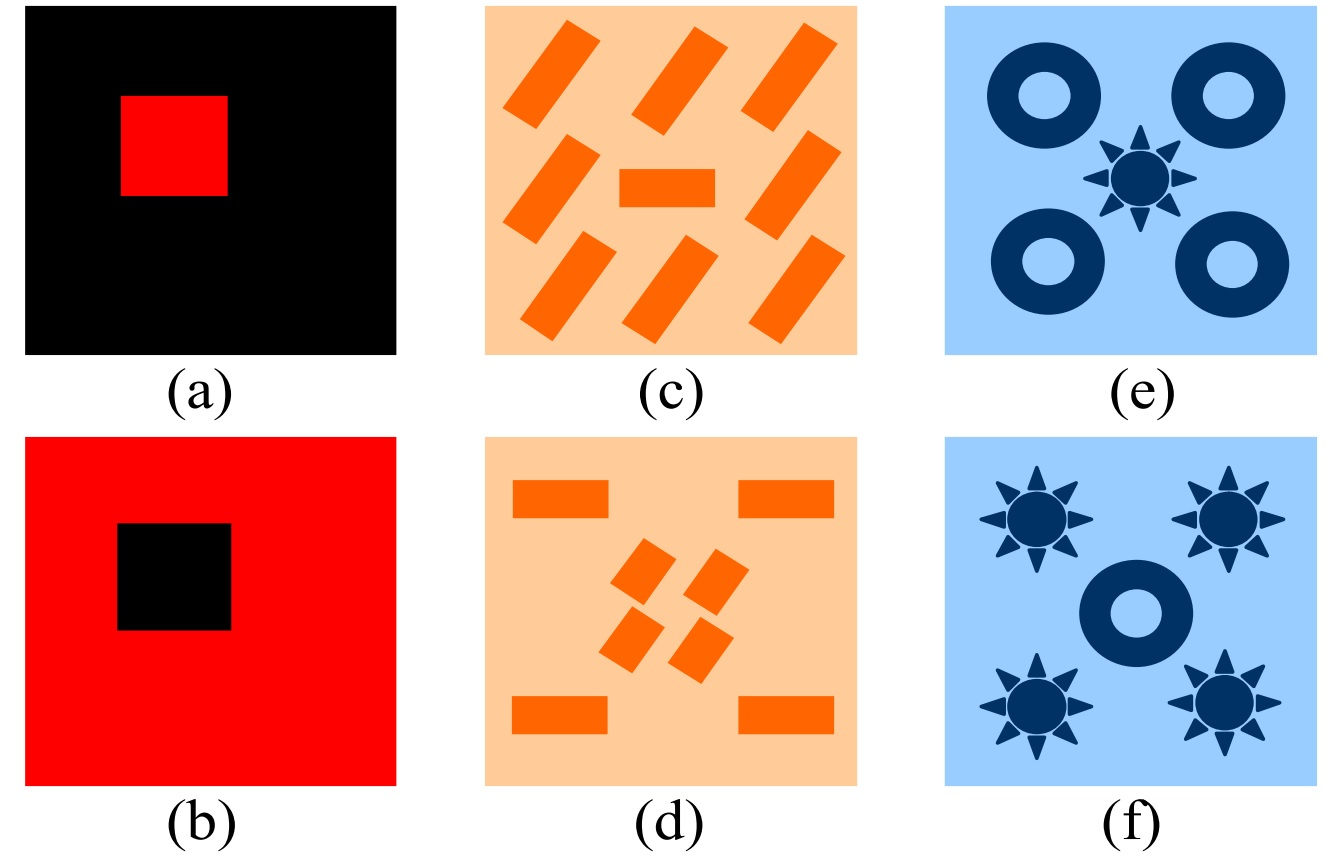
\includegraphics[width=\textwidth]{local_contrast.jpg}
\caption{对比度在视觉感知中的作用}\label{fig:local_contrast}
\end{figure}

传统的图像处理技术通常只考虑了颜色、纹理和形状这三个基本特征,然而,对比度在视觉感知中的重要作用却常常被人们所忽略。以下这个例子可以说明对比度的重要性\citep{ma2003contrast},如图\ref{fig:local_contrast}所示的三组图像,在图\ref{fig:local_contrast}(a)中,有一个红色的方形盒子被黑色的背景所围绕。很显然,红色盒子所在区域更容易吸引人们的注意力,对这个现象的一个解释是,因为红色是一种更容易引起人们视觉注意力的鲜艳色彩。然而,图\ref{fig:local_contrast}(b)却无法支持这个假设,显然在这幅图像中,黑色的区域成为了吸引人们注意力的区域。这个现象表明,尽管颜色能够影响人们的视觉感知,但是却并非影响视觉注意力最重要的因素。图\ref{fig:local_contrast}(c)(d) 展示了两幅有一定纹理方向的图像,类似(a)(b)两图,说明了纹理并非视觉感知中最重要的因素。图\ref{fig:local_contrast}(e)(f)则说明了形状在视觉感知中的作用。然而,以上三组图像都有一个共同的特征,那就是,显著区域通常被背景区域围绕并呈现高对比度(无论是颜色、纹理还是形状上的高对比度),这在一定程度上说明了高对比度的物体通常能吸引人眼的注意力。基于局部对比度的方法利用了图像区域相对于(一个小的)局部邻域的稀缺度来检测显著性区域。在此定义下,检测子的形式通常表现为“中心-周围差异”,不同方法的变化在于:1)尺度问题(即“中心-周围差异”中,“周围”的大小);2)差异的度量问题(在哪种特征空间下比较、周围像素点的权值等)。本节以MZ\cite{ma2003contrast}方法为例,介绍基于局部对比度的方法。在MZ中,局部对比度被定义为:
\begin{equation}
C_{i,j} = \sum_{q \in \Theta}d(p_{i,j},q) \label{eq:local}
\end{equation}

其中,$c_{i,j}$代表在$(i,j)$位置的像素点的对比度,$p_(i,j)$代表该像素点的某种特征向量(例如颜色向量),$q$代表周围像素点的特征向量,$d(x,y)$表示$p_{i,j}$与$q$的差异,通常使用欧式距离度量,$\Theta$即代表周围像素点的集合,通过控制$\Theta$的大小,即可控制“感知域”的大小。最后,将所有图像像素对比度的值归一化到0,1之间,即得到像素的显著值。可以看出,这个定义下,一个像素点的显著值实际上就是它与周围像素点的差异和。

基于公式\ref{eq:local},衍生出了一些其他方案:1)通过调整$\Theta$的范围,就可以调整检测子的尺度。近期的一些工作,已经不满足于通常的矩形或圆形邻域,开始寻找一些特性更好的邻域(比如邻域边界与图像边缘一致的邻域)。2)改换特征空间,比如在梯度空间下,或者其他自定义的特征空间。3)加入权值,公式\ref{eq:local}认为周围像素点对中心像素点的贡献是一样的(权值都为1),而另外一些研究者认为,与中心像素点距离近的像素对其对比度的贡献更高,所以对距离中心近的像素点赋更大的权值。

上面的讨论给出了基于局部对比度的显著区域检测方法的核心思想。然而,该类方法有一个严重的缺陷,它倾向于给物体边缘赋予较大的显著值(因为物体边缘的“中心-周围差异度”通常较大)。在较小的尺度下,检测子近似退化为一个边缘检测算子。

\section{基于全局对比度的方法}
基于局部对比度的方法,倾向于给物体边缘赋予较大的显著值,而无法均匀的高亮整个显著区域。研究者发现,采用全局对比度计算显著图可以解决这个问题。相比基于局部对比度的方法,基于全局对比度的方法能够均匀的高亮整个显著性区域而非边缘,原因是,在全局环境下(即将像素点的邻域扩展到全图),具有相同特征的像素(如颜色)必然被赋予相同的显著值。Zhai\cite{zhai2006visual}等人早在2006年就提出了基于全局对比度的显著区域检测算法,考虑到计算复杂度的问题,他们仅仅采用了像素的亮度值来计算像素点之间的差异。随后Cheng\cite{cheng2011global}等人提出,利用三个颜色通道度量像素点的差异更加有利于显著区域检测性能的提高,在HC方法中,一个像素点$I_k$的显著值定义为:
\begin{equation}
S(I_k)=\sum_{\forall I_i \in I}D(I_k,I_i)
\end{equation}

其中,$I$代表整个图像像素点的集合,$I_i$代表第$i$个像素点在Lab颜色空间的颜色向量,$D(*,*)$为欧式距离算子。在该式中,颜色相同的像素必然会得到相同的显著值,为了进一步减少计算开销,可将上式进一步简化为:
\begin{equation}
S(I_k)=S(c_l)=\sum_{j=1}^n f_j D(c_l,c_j)
\end{equation}

其中,$c_l$代表像素$I_k$的颜色向量,$c_j$代表第$j$个颜色的颜色向量,$f_j$代表第$j$种颜色在整个图像中出现的频率。经分析可知,计算上式的时间复杂度为$O(N)+O(n^2)$,$N$为像素的个数,$n$为整个图像中不同颜色的数量。在不经过任何优化的情况下,原颜色空间的颜色个数为$n=256^3$,这样的时间复杂度是不可忍受的。因此,Cheng首先将每个颜色通道量化为12个值,这样颜色的数量下降为$n=12^3=1728$。
\begin{figure}
\centering
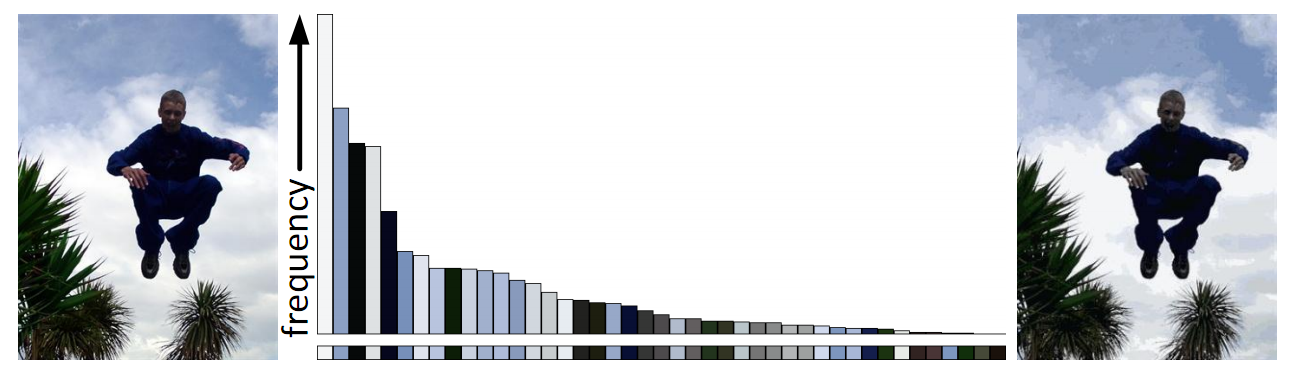
\includegraphics[width=\textwidth]{global_contrast.png}
\caption{使用少量高频颜色量化图像}\label{fig:global_contrast}
\end{figure}
进一步的,如图\ref{fig:global_contrast}所示,忽略占像素数量较少的颜色,使用出现频率高的颜色替代,使得剩余的颜色占到像素数量的$95\%$,颜色的数量可以进一步下降到$85$左右(忽略的颜色使用剩余颜色中最相近的代替),同时基本不影响图像的主观视觉质量\cite{cheng2011global},这样就大大降低了算法的时间复杂度。然而,通过该方法优化性能,会给图像带来很明显的量化痕迹(原本非常相近的两个颜色,可能会被量化到不同的值)。因此,为了进一步优化检测效果,Cheng另外引入了颜色空间平滑,即对相近颜色的显著值进行了加权平均,具体做法如下:
\begin{equation}
S'(c) = \frac{1}{(m-1)T}\sum_{i=1}^{m}(T-D(c,c_i))S(c_i)
\end{equation}

其中,$T=\sum_{i=1}^m D(c,c_i)$是颜色$c$与最相近的m种颜色的距离和。论文中还介绍了RC方法,即Region Based Contrast,该方法首先使用一般的分割方法将图像分割为许多区域,然后使用该区域的平均颜色作为区域的颜色值,最后使用相似的方法,以区域为基本计算单元,计算区域的全局对比度。

\section{基于频域分析的方法}
基于频域分析的方法将图像转化到频域处理,并结合信息压缩理论,将图像中“新颖”的频率部分分离出来,最后再转回空间域。这里以SR\cite{hou2007saliency}为例进行分析。在信息压缩理论中,一幅图像的信息量可以被分解为两部分:
\begin{equation}
H(Image)=H(Innovation)+H(Prior Knowledge)
\end{equation}

对于$H(Prior knowledge)$是我们已知的一些先验知识,所以无需编码,只需对$H(Innovation)$这部分进行编码传输即可。解码时,由于先验知识已知,我们通过解码$H(Innovation)$这部分,就可以恢复原图像,从而达到信息压缩的目的。而显著性区域即对应$H(Innovation)$这部分内容,这就是基于频域处理方法的理论基础。

\begin{figure}[h]
\centering
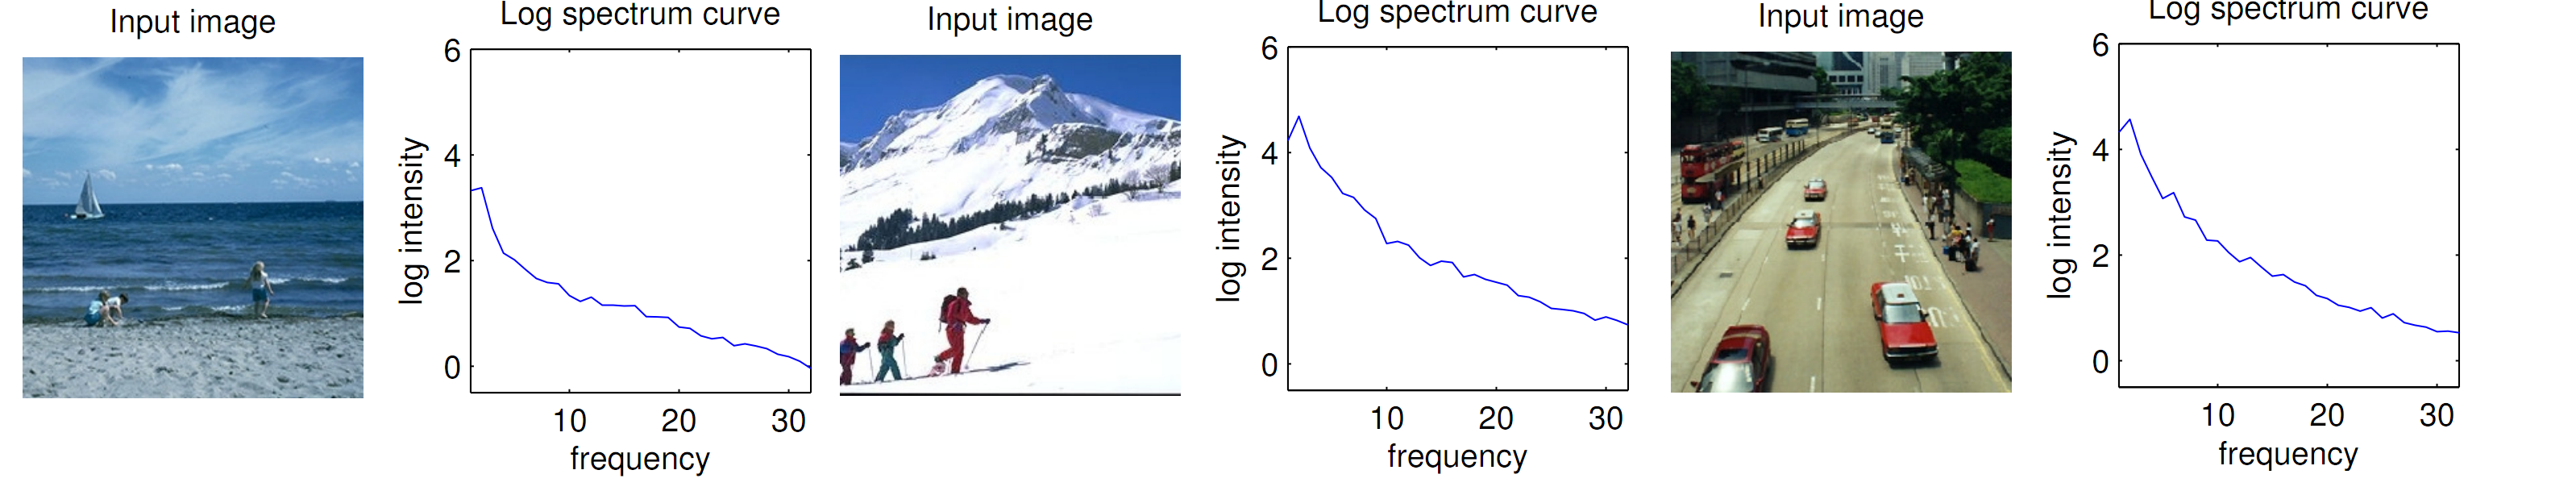
\includegraphics[width=\textwidth]{log_spectrum.png}
\caption{不同图像的log spectrum呈现为相似的曲线}\label{fig:log_spectrum}
\end{figure}

\begin{figure}[t]
\centering
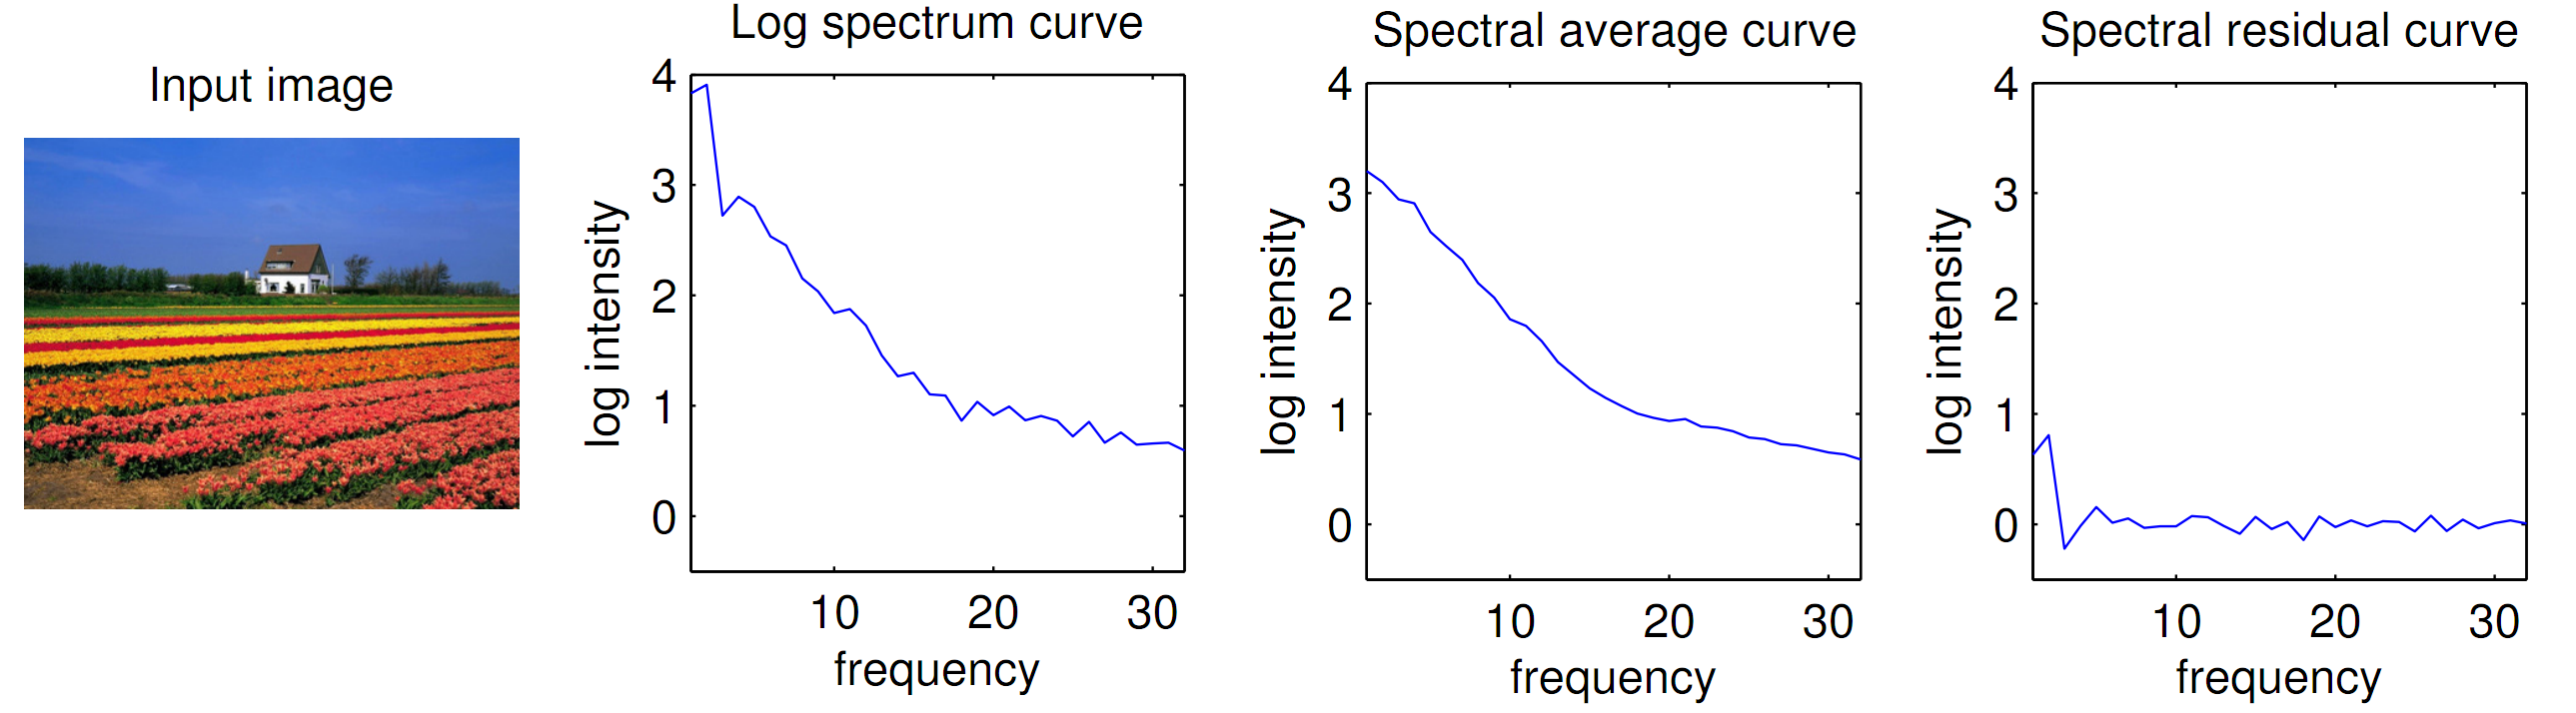
\includegraphics[width=\textwidth]{frequency_residual.png}
\caption{通过求得log spectrum的残差得到显著区域}\label{fig:frequency_residual}
\end{figure}

论文指出,图像的log spectrum具有相似的变化曲线,如图\ref{fig:log_spectrum}所示,此曲线即对应的先验知识,因此通过求训练图像log spectrum曲线的均值,我们就可以得到图像在频率域的“先验知识”。如图\ref{fig:frequency_residual}所示,将待检测图像的log spectrum减去先验,得到的残差值,即为显著区域对应的频域表达,再通过逆变化,变换到时域,即可得到显著图。

然而有文章\cite{hou2012image}指出,基于频域分析的方法实际上等同于基于局部对比度的方法加上一个高斯模糊,因此与基于局部对比度的方法具有相同的缺陷,在大尺度图像中,容易高亮物体的边缘。

\section{基于学习的方法}
这里介绍Mai等人\cite{maisaliency}提出的使用条件随机场(CRF)的模型。作者提出,目前已经存在许多经典的显著区域检测算法,各类方法针对不同的场景都会有一定的效果,如果能有效的将这些方法融合起来,相互补充,就能产生高质量的显著图。如图\ref{fig:crf_learn}所示,(c)(d)(e)(f)四种方法均能取得一定的显著区域检测效果,但是都有各自的缺陷,比如(f)只高亮了显著区域的边缘,而(e)方法对显著和非显著区域的区分不明显。Mai等人通过条件随机场(CRF)融合多种方法,产生如图\ref{fig:crf_learn}(g)(h)所示的显著图,可以看到CRF和CRF-GIST方法取得了良好的检测效果。通过融合多特征产生高质量显著图的思想,在Borji的工作中\cite{borji2012salient}也有所涉及,只是在Borji的文章中,结合多种特征的方式比较简单,即采用简单的加权平均,或者对应像素相乘等等。Mai等人指出\cite{maisaliency},简单的相加相乘并没有考虑到相邻像素之间的关联性,通过加入空间位置信息(相邻且相似的像素的显著性应该比较接近),可以取得更好的融合效果。

\begin{figure}[h]
\centering
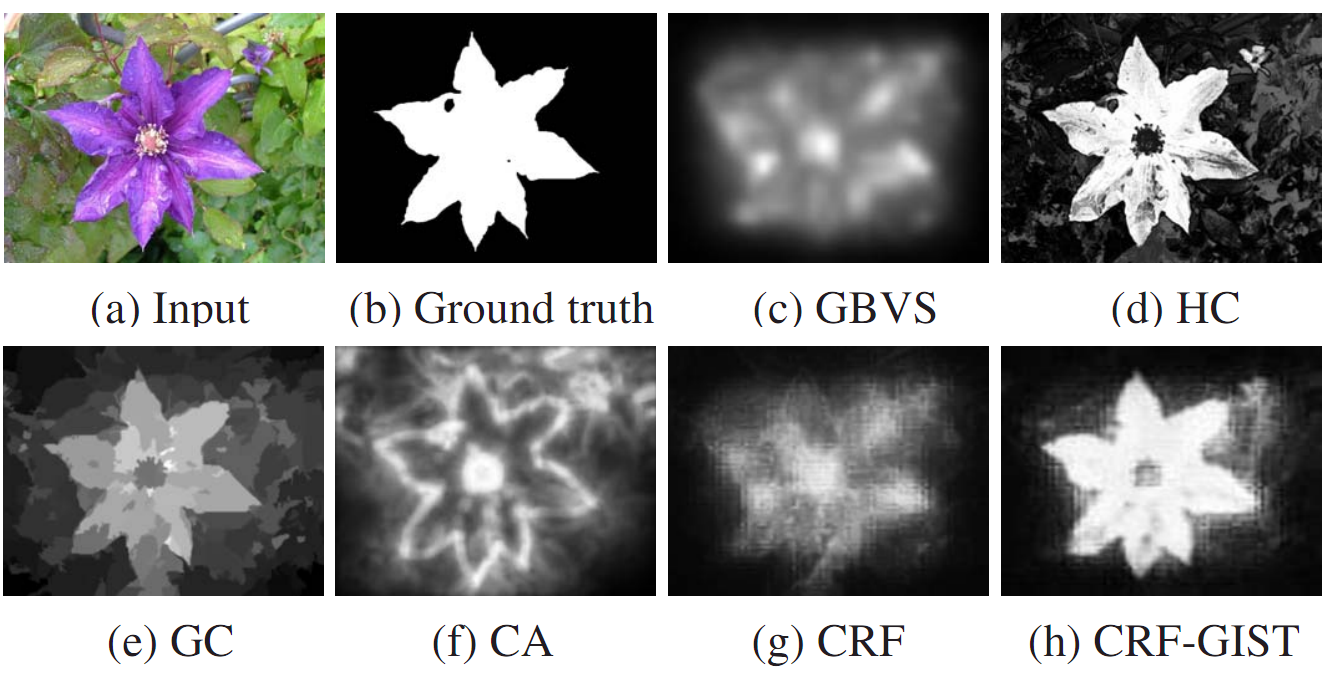
\includegraphics[width=\textwidth]{crf_learn.png}
\caption{结合多个显著图}\label{fig:crf_learn}
\end{figure}

在Mai的模型中,给定一幅图像$I$,我们使用一个二值掩图$Y=\{y_p|p\in I\}$来标出显著物体。在CRF模型中,以每个像素点为顶点,8领域像素点之间相连,形成一个晶格状的图。那么,在这个图下,$Y$在给定图像$I$下的条件概率可以写为,
\begin{equation}
P(Y|I) = \frac{1}{Z}exp(\sum_{p\in I}F_d(y_p, I) + \sum_{p\in I}\sum_{q\in N_p}F_s(y_p,y_q,I) )
\end{equation}

其中,$p$代表$I$中的一个像素点,$y_p$是其显著与否的标记。$F_d(y_p, I)$是node feature function,$F_s(y_p,y_q,I)$是edge feature function,描述了相邻像素点之间的联系。

Node feature function仅仅与输入的已有显著图$S_i$有关,即
\begin{equation}
F_d(y_p, I) = \sum_{i=1}^{m} \lambda_iS_i(p) + \lambda_{m+1}y_p
\end{equation}

其中,$\lambda_i$是条件随机场的一组待学习的参数。Edge feature function描述了相邻像素之间的关系:
\begin{equation}
F_s(y_p,y_q,I) = F_e(y_p,y_q,I) + F_c(y_p,y_q,I)
\end{equation}

其中,$F_e(y_p,y_q,I)$考虑到了这样一个事实,如果两个像素点在同一幅显著图中的显著值差别很大,那么算法倾向于赋予它们不同的显著值。
\begin{equation}
  F_e(y_p,y_q,I) = \sum_{i=1}^{m}\alpha_i(\textbf{1}(y_p=1,y_q=0)-\textbf{1}(y_p=0,y_q=1))(S_i(p)-S_i(q))
\end{equation}

其中,$\alpha_i$为CRF的待学习参数,$\textbf{1}(.)$为指示函数(括号内真为1,假为0)。$F_s$的第二项可以看做一个惩罚项,当像素点的颜色相似却被标上不同的标记时要进行惩罚:
\begin{equation}
F_c(y_p,y_q,I)=\textbf{1}(y_p \not= y_q) exp(-\beta \parallel I(p)-I(q) \parallel )
\end{equation}

其中,$\parallel I(p)-I(q) \parallel$代表像素$p$和$q$的颜色差(Lab颜色空间),$\beta$被设置为$(2<\parallel I(p)-I(q) \parallel>^2)^{-1}$,$<.>$代表计算期望。

最后,通过训练这个模型,得到所有参数的最优值。当计算新的显著图时,我们取每个顶点(像素点)被标记为1的边缘概率作为该像素点的显著值。

可以看出,基于学习的方法原理较为复杂,同时离线训练和在线检测都比较耗时。另外,\citep{liu2011learning}指出,基于学习的方法十分依赖训练数据集,因此在不同的数据集合上,表现差异较大。

\section{最新工作与研究趋势}
除了以上介绍的一些经典方法,近年来在该领域也出现了许多新颖且实用的工作\cite{borji2012salient}\cite{yan2013hierarchical}\cite{shi2013pisa}\cite{wei2012geodesic},研究者们对显著性区域检测的研究方向有了如下一些共识和趋势:
\begin{itemize}
\item 多尺度,多特征的融合。在小尺度下,一些面积很小但对比度高的区域很容易造成显著图质量的下降,在大尺度下,虽然可以屏蔽这些区域的影响,但是检测的粒度又会变得十分粗糙。因此,有必要结合多个尺度,以提高检测的精度和鲁棒度。另外,单一的特征都有其适用范围,往往只在特定的场景下起到特定的作用,因此融合多个特征(颜色,纹理等等)以提高检测精度也变的十分重要。
\item 趋向于基于区域的特征。基于点的特征对噪声敏感,而基于区域的特征则可以更加鲁棒的提取出该区域的特性。值得注意的是,近的许多工作都使用了SLIC\cite{achanta2010slic}这个超像素分割算法,将空间上近似的像素点分割为一个小的区域进行计算。
\item 加入一些更高层的特征。底层特征在简单场景下有良好的效果,但是在复杂场景下性能下降明显,加入高层特征(如人脸识别子,汽车识别子等等)有助于改善显著区域检测结果。
\item 将时间复杂度作为一项重要的考察指标。作为一项预处理技术,显著区域检测的时间复杂度决定了其实用价值。
\end{itemize}

\section{本文研究框架与思路}
\begin{figure}[h]
\centering
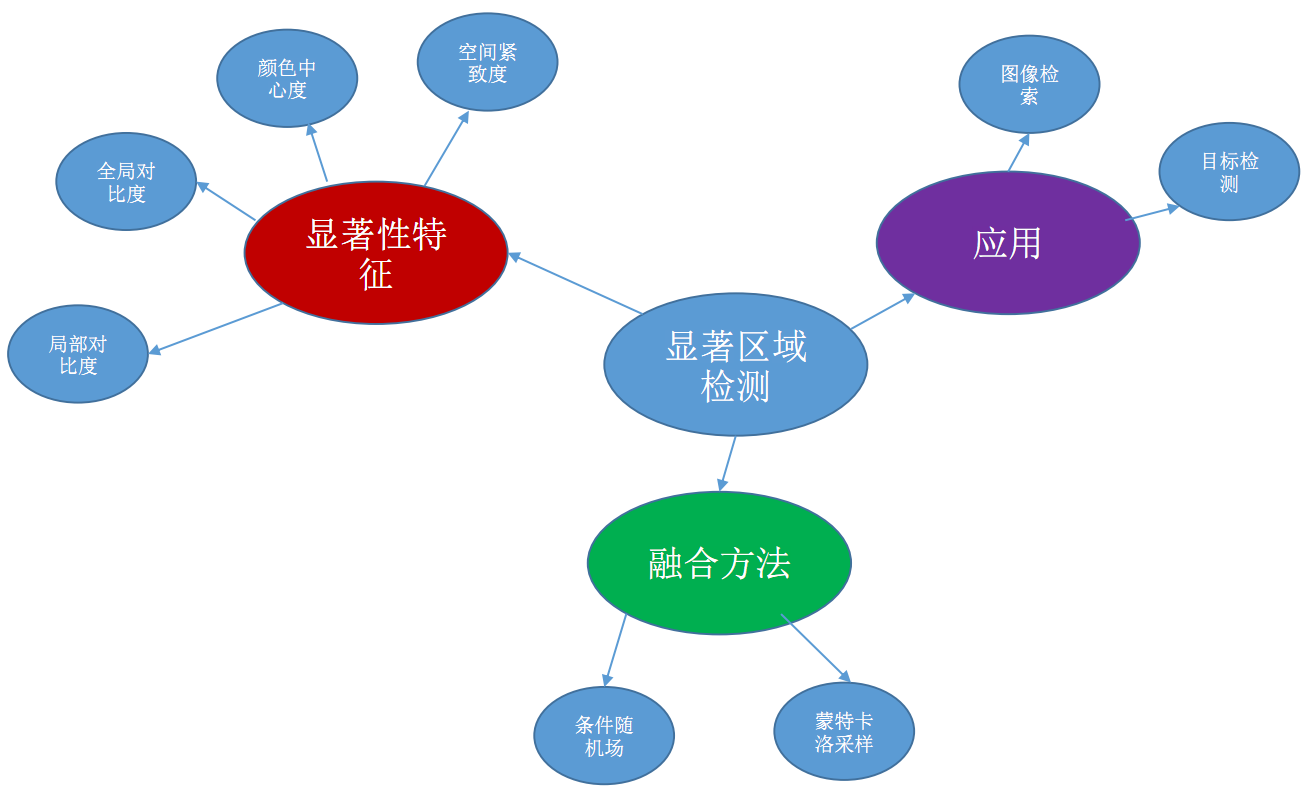
\includegraphics[width=\textwidth]{framework.png}
\caption{研究框架图} \label{fig:framework}
\end{figure}

尽管研究者们已经对显著区域检测做出了各种各样的尝试,但该领域仍然存在许多尚待解决的问题:首先,人们对视觉注意力的形成机制还未研究透彻,目前获得大家共同认可的对比度注意力机制也只能在一定的场景下发挥作用,还需要发掘更多的显著性特征以帮助算法更好的进行显著区域的检测;其次,目前已经存在许多针对不同先验、场景和底层信息的显著区域检测算法,这些算法各有优劣,产生的显著图也不尽相同,各有补充,如何有机将这些方法融合起来,产生更高质量的显著图,这也是一个重要的课题;最后,显著区域检测作为一项预处理技术,必须与其他任务相结合才能体现其价值,然而现有的研究工作大多将显著区域检测应用于图像分割任务,并将分割的结果作为评价算法优劣的指标,但是在分割任务中表现突出的算法,不一定适用于其他任务(如图像检索、目标检测等),因此显著区域检测算法在其他应用场景中的表现,也是亟待评估和研究的。

为了解决上述问题,本文按照如图\ref{fig:framework}所示的框架,针对显著区域检测的机制、模型和算法以及应用开展针对性研究,主要探索了显著性特征、融合方法及其应用。我们具体的研究思路如下:
\begin{enumerate}
\item 首先解决人眼视觉注意力的机制,即什么样的图像区域能引起人眼的视觉注意(显著性特征)。我们提出了多个符合人眼视觉注意力机制的,且可计算的显著性特征,包括局部对比度、全局对比度、颜色中心度、空间紧致度等等。
\item 接着解决多特征融合的问题。各个特征都具有特定场景下的特定意义,因此将这些特征结合起来,产生互补效应以提高检测效果,是非常重要的。针对不同的应用场景和需求,我们提出了条件随机场和蒙特卡洛采样两种特征融合方法。
\item 最后,我们解决显著区域检测的应用问题。显著区域检测作为一项计算机视觉的预处理技术,如果无法应用于实际场景中,将失去其存在的价值。我们重点研究了显著区域检测在图像检索中的应用。
\end{enumerate}

\section{本章小结}
本章介绍了显著性区域检测的四类经典算法:基于局部对比度、基于全局对比度、基于频域分析和基于学习的方法。基于局部对比度的方法符合人类对生物视觉的认知,然而却容易高亮区域边缘;基于全局对比度的方法则改良了上述缺点,能较好的高亮整个显著区域;基于频域分析的方法拥有良好的理论基础,但是其处理效果同基于局部对比度的方法一样,容易强调边缘的显著度;最后基于学习的方法能有效的结合各类特征,得到良好的效果,但是其训练时间过长,且与数据相关。另外,还介绍了国际上关于该课题最新的一些思路和研究趋势,这为我们未来的工作指明了方向。在本章的最后,我们提出了自己的研究框架与思路,在接下来的章节中,我们将按照该框架展开我们的研究工作。
